\subsection{Prise de données à CMS}\label{chapter-LHC-section-CMS-subsec-data_taking}
Pour un événement, le détecteur CMS décrit dans les sections précédentes produit une quantité de données de l'ordre de \SI{1}{\mega o}.
Si cette grandeur peut paraître raisonnable, il faut la mettre en relation avec la fréquence des événements.
Des collisions ont lieu toutes les \SI{25}{\nano\second} au LHC, soit à une fréquence de \SI{40}{\mega\hertz}.
Le détecteur CMS produit alors un flux de données de \SI{40}{\tera o.\second^{-1}}, ce qui est bien trop important, tant pour l'électronique d'acquisition que pour la reconstruction des événements, abordée section~\ref{chapter-LHC-section-evt_reco}, et pour la quantité de données à stocker elle-même.
Afin d'en réduire le débit, la collaboration CMS s'appuie sur un système de déclenchement (\emph{trigger})~\cite{cms_paper,CERN-LHCC-2000-038,CERN-LHCC-2002-026,CMS-TRG-12-001,CMS-TDR-12} dont le rôle est de supprimer les événements présentant peu d'intérêt physique.
\par Le système de déclenchement de CMS comporte deux niveaux, le niveau \og L1 \fg{} (\emph{Level-1}) et le niveau \og HLT \fg{} (\emph{High Level Trigger}).
Le L1 est constitué d'un système électronique programmable utilisant les signaux issus des chambres à muons et des calorimètres pour estimer l'intérêt d'un événement, par exemple par la présence de muons ou d'activité calorimétrique.
Il doit analyser chacun des événements.
Ceux ne présentant ni muons ni activité calorimétrique suffisante sont directement rejetés.
En revanche, jusqu'à \SI{3.2}{\micro\second} sont nécessaires au traitement des événements les plus complexes~\cite{cms_paper}.
Un système de mise en attente est donc utilisé.
Le L1 permet ainsi de réduire la fréquence des événements à analyser de \SI{40}{\mega\hertz} à \SI{100}{\kilo\hertz}, limite imposée par l'électronique de lecture complète du détecteur~\cite{CMS-TRG-12-001}.
La structure du L1 est illustrée sur la figure~\ref{fig-chapter-LHC-section-CMS-subsec-data_taking-cms_paper-fig_8-1}.
\begin{figure}[h]
\centering
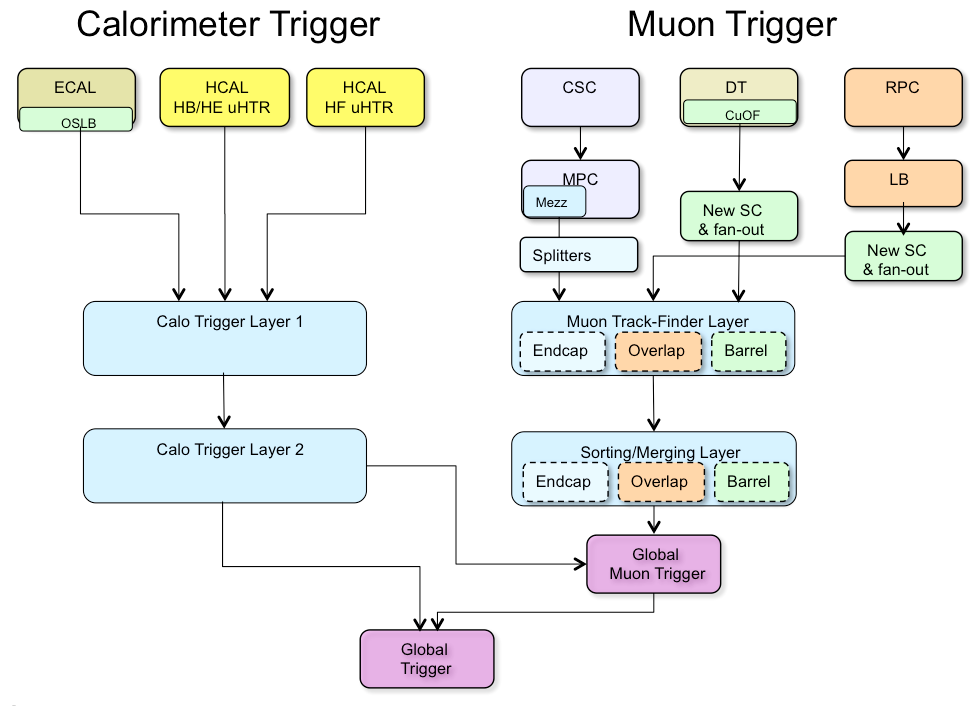
\includegraphics[width=\textwidth]{\PhDthesisdir/plots_and_images/from_CMS-TDR-12/L1_structure.png}
\caption[Architecture du système de déclenchement L1.]{Architecture du système de déclenchement L1~\cite{CMS-TDR-12}.}
\label{fig-chapter-LHC-section-CMS-subsec-data_taking-cms_paper-fig_8-1}
\end{figure}
\par Le second niveau de déclenchement, le HLT, a accès à l'ensemble des signaux issus du détecteur.
Une reconstruction simple des événements est réalisée sur une ferme de calcul et permet d'identifier les photons, muons, électrons, jets et taus hadroniques de l'événement.
Des calculs plus complexes, similaires à ceux utilisés dans les analyses finales, sont alors réalisés~\cite{cms_paper}.
Il est possible de concevoir de nombreuses conditions de sélection sur les particules présentes, leur énergie, etc.
Il existe ainsi de nombreux chemins de déclenchement (HLT \emph{paths}).
La reconstruction simple des événements et leur sélection se fait en un temps maximal de \SI{50}{\milli\second}.
La fréquence moyenne des événements conservés est ainsi abaissée à \SI{100}{\hertz}~\cite{cms_paper,CMS-TRG-12-001}, fréquence raisonnable pour enregistrer les données.